\clearpage
\setcounter{page}{1}
\maketitlesupplementary



\section{Dataset Details}




This section provides comprehensive information about our experimental datasets, including data characteristics, annotation details, acquisition protocols, and their roles in our experimental setup. We describe both the datasets used for upstream training and those held-out for out-of-distribution evaluation.



\noindent\textbf{Multi-organ Abdominal Collection (AMOS).} AMOS~\cite{ji2022amos} represents a comprehensive multi-modal dataset from Longgang District People's Hospital, featuring 500 CT and 100 MRI scans from 600 patients with abdominal abnormalities. Acquired across eight different scanner platforms, the dataset provides annotations for 15 anatomical structures, including major abdominal organs, vessels, and reproductive organs: spleen, right kidney, left kidney, gallbladder, esophagus, liver, stomach, aorta, inferior vena cava, pancreas, right adrenal gland, left adrenal gland, duodenum, bladder, and prostate/uterus. The CT portion offers 200 training and 100 validation scans, while the MRI section provides 40 training and 20 validation scans. We employ both modalities in upstream training, using a 95/5 split for training/validation using the official training set, while using the official validation set for evaluation. Note that the MRI validation set lacks bladder and prostate annotations, limiting MRI segmentation to 13 structures.


\noindent\textbf{Whole-body PET/CT Collection (AutoPET).} AutoPET~\cite{gatidis2022whole} represents a comprehensive collection of 1014 whole-body FDG-PET/CT studies, balanced between 501 cases with confirmed malignancies (lymphoma, melanoma, NSCLC) and 513 negative control cases. All scans include both PET and CT modalities, making it valuable for multi-modal analysis. We maintain patient-level data integrity with a 75\%/5\%/20\% split for training, validation, and testing.


\noindent\textbf{Abdominal CT from Multi-Atlas (BCV).} The BCV~\cite{bcv}  collection consists of 50 abdominal CT scans obtained during routine clinical care at Vanderbilt University Medical Center (VUMC). Of these, 30 scans are publicly accessible with volumetric annotations of 13 abdominal organs created using MIPAV software. The annotated structures encompass major organs and vessels including the liver, kidneys (left/right), pancreas, spleen, gallbladder, esophagus, stomach, aorta, inferior vena cava, portal and splenic veins, and adrenal glands (left/right). Notable is the occasional absence of right kidney or gallbladder annotations in some patients. For our upstream training pipeline, we implement a 75\%/5\%/20\% split of the available data for training, validation, and testing respectively.


\noindent\textbf{Brain Aging Study Collection (Brain)~\cite{rodrigue2012beta}.} Part of the Dallas Lifespan Brain Study, this dataset aims to understand cognitive function changes across adult life, particularly focusing on early indicators of Alzheimer's Disease progression. Our analysis utilizes 213 T1-weighted MRI scans, annotated for three key brain tissue types: cerebrospinal fluid, gray matter, and white matter. Following established protocols~\cite{rao2022improving}, we distribute the scans into 129 training, 43 validation, and 43 testing cases.

\noindent\textbf{Abdominal MRI Collection (CHAOS).} CHAOS~\cite{CHAOS2021} focuses on precise abdominal organ segmentation in magnetic resonance imaging. The dataset features multi-sequence MRI scans (T1-in-phase, T1-out-phase, T2-SPIR) from 20 patients, with annotations of four major abdominal organs: liver,  left kidney, right kidney, and spleen. Each MR sequence is treated as an independent image for analysis purposes, while maintaining patient-level data splits of 75/5/20 for training, validation, and testing to prevent data leakage.

\noindent\textbf{Kidney Tumor Dataset (KiTS19)~\cite{heller2019kits19}.} Sourced from the University of Minnesota Medical Center between 2010-2018, KiTS19 comprises CT scans and treatment outcomes from 300 kidney tumor patients who underwent nephrectomy procedures. The publicly available portion includes 210 cases, while 90 remain private for evaluation purposes. We incorporate this dataset into our upstream training using a 75\%/5\%/20\% of the 210 training cases for training/validation/testing.




\noindent\textbf{Liver Cancer Imaging Collection (LiTS)~\cite{bilic2019liver}.} This dataset encompasses 201 abdominal CT scans (131 training, 70 testing) gathered from seven prominent medical institutions including centers in Munich, Nijmegen, Montreal, Tel Aviv, and Strasbourg. The collection features patients with various liver malignancies, including primary hepatocellular carcinoma and metastases from colorectal, breast, and lung cancers. The scans exhibit diverse tumor characteristics and contrast enhancement patterns, captured both pre- and post-treatment using various CT protocols. Annotations include detailed tumor delineation alongside broader liver segmentation. We utilize the 131 public training cases with a 75\%/5\%/20\% split for our upstream training framework.



\noindent\textbf{Cardiac MRI Dataset (M\&Ms).} The M\&Ms~\cite{campello2021multi} dataset represents a diverse cardiac imaging collection from the MICCAI 2020 Challenge, featuring scans from patients with cardiomyopathies (both hypertrophic and dilated) and healthy controls. Its unique strength lies in its multi-center (three countries: Spain, Germany, Canada) and multi-vendor (Siemens, GE, Philips, Canon) acquisition protocol. The dataset comprises 150 annotated training images equally distributed across two vendors, and 170 testing cases spread across all four vendors (20 from one vendor, 50 each from three others). Annotations include left ventricle, right ventricle, and left ventricular myocardium at both end-diastolic and end-systolic phases. We utilize the official test set for evaluation and split the training data 95\%/5\% for training and validation.





\noindent\textbf{Radiation Treatment Planning Dataset (StructSeg).} StructSeg~\cite{structseg} comprises specialized CT imaging data focused on radiation therapy planning for nasopharynx and lung cancers. The collection is divided into two primary components: head \& neck (StructSeg H\&N) and thoracic (StructSeg Tho) imaging. The head \& neck portion includes scans from 50 nasopharynx cancer patients with detailed annotations of 22 organs-at-risk (OARs), encompassing crucial structures such as ocular components, brain regions, and maxillofacial structures. The 22 OARs are: left eye, right eye, left lens, right lens, left optical nerve, right optical nerve, optical chiasma, pituitary, brain stem, left temporal lobes, right temporal lobes, spinal cord, left parotid gland, right parotid gland, left inner ear, right inner ear, left middle ear, right middle ear, left temporomandibular joint, right temporomandibular joint, left mandible and right mandible. The thoracic component contains scans from 50 lung cancer patients with annotations of six critical OARs: left lung, right lung,, spinal cord, esophagus, heart, and trachea. We implement a consistent 75\%/5\%/20\%  division for training, validation, and testing across both components.



\noindent\textbf{Spine Imaging dataset (CSI).} CSI~\cite{ivdm3seg} dataset is a specialized collection from the MICCAI Workshop Challenge on Spine Imaging, comprising multi-modal MRI scans of intervertebra discs. The dataset contains 16 complete 3D MRI sets using a Siemens 1.5-Tesla scanner with Dixon protocol, each scan generates four aligned high-resolution 3D volumes (in-phase, opposed-phase, fat, and water images). The imaging focuses on the lower spine, capturing at least 7 intervertebral discs (IVDs) per subject, with expert-annotated binary masks provided for each IVD. We use the four MR modality as separate datasets, namely CSI-inn, CSI-opp, CSI-fat and CSI-wat. The illustration of these four modalities are shown in Figure~\ref{fig:supp_csi}.  We use the CSI-wat in the upstream training, and testing the trained model on CSI-inn, CSI-opp, CSI-fat to evaluate the generalization capability. We can observe that CSI-opp and CSI-inn has relatively similar appearence, where CSI-fat has totally contradictory contrast and intensity, showing great distribution gap.


\begin{figure}[ht]
\begin{center}
%\framebox[4.0in]{$\;$}
%\fbox{\rule[-.5cm]{0cm}{4cm} \rule[-.5cm]{4cm}{0cm}}
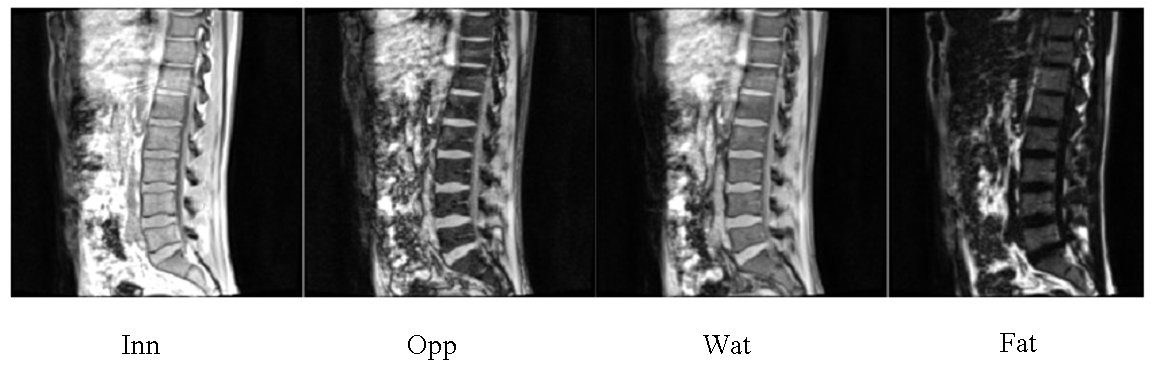
\includegraphics[width=\columnwidth]{./fig/supp_csi.pdf}
\end{center}
\vspace{-1em}
\caption{Illustration of four MR modalities of the CSI dataset.}
\label{fig:supp_csi}
\vspace{-1em}
\end{figure}


\noindent\textbf{Automated Cardiac Diagnosis Dataset (ACDC).} The ACDC dataset~\cite{bernard2018deep} consists of cardiac MRI scans collected at the University Hospital of Dijon, covering various cardiac conditions including normal subjects and four pathological groups (myocardial infarction, dilated cardiomyopathy, hypertrophic cardiomyopathy, and right ventricle abnormalities). The scans were acquired using two different Siemens MRI scanners (1.5T and 3.0T) over a six-year period, providing short-axis cardiac images with expert annotations at end-systolic (ES) and end-diastolic (ED) phases. We utilize 100 cases from this collection as a downstream evaluation task to assess our model's generalization capability from the M\&Ms dataset, as they represent different medical centers and scanner configurations while sharing similar anatomical targets.




\noindent\textbf{Thoracic Risk Organ Dataset (SegTHOR).} SegTHOR~\cite{lambert2020segthor} focuses on thoracic organ-at-risk segmentation, providing 40 CT scans with annotations of four critical structures: heart, aorta, trachea, and esophagus. SegTHOR serves as a downstream evaluation task to assess model generalization from StructSeg Tho. We evaluate upstream-trained models directly on all 40 images without additional training.

\noindent\textbf{MSD pancreas \& tumor dataset.}
The MSD pancreas \& tumor dataset is a part of the Medical Image Segmentation Decathlon (MSD)~\cite{antonelli2022medical}, an international challenge aimed at identifying a general-purpose algorithm for medical image segmentation. The competition encompasses ten distinct datasets featuring various target regions, modalities, and challenging attributes. MSD pancreas \& tumor is one of the datasets that is annotated for pancreas and tumors. The shape and position of tumors vary greatly between patients. The MSD pancreas \& tumor dataset consists of 281 CT images. We use it as a downstream task to evaluate models' ability to handle unseen classes, we only use the tumor class for evaluation. We split this dataset into 75\%/5\%/20\% as context/validation/testing set.


\noindent\textbf{Pelvic CT Dataset (Pelvic).} The Pelvic1K dataset~\cite{liu2021deep} is a comprehensive collection of CT scans aggregated from multiple sources, including clinical cases (pre- and post-operative pelvic fractures) and public datasets . These diverse sources provide images with varying field of view, spacing, and clinical conditions, including cases with metal artifacts, vascular sclerosis, and other clinically relevant variations. For our evaluation, we utilize the subset (dataset 6) of Pelvic1K with 103 CT scans with annotations of four skeletal structures: sacrum, left hip bones, right hip bones and lumbar spine. We employ this dataset as a downstream task to assess model performance on novel anatomical structures, using a 75\%/5\%/20\% split for context, validation, and testing respectively.

\begin{table}
  \caption{Datasets statistics. The upper datasets are for upstream training and analysis. The bottom datasets are for downstream tasks on generalization and unseen classes.}
  \label{tab:dataset}
  \centering
   \scriptsize
   \setlength{\tabcolsep}{0.8mm}{
  \begin{tabular}{ccccccc}
    \toprule
    Dataset         & Body Region   & Modality  & Clinical Target   & \#Cls &   Size     \\
    \midrule
    AMOS CT~\cite{ji2022amos}  & Abdomen       & CT        & Organs            & 15        & 300   \\
    AMOS MR~\cite{ji2022amos}  & Abdomen       & MRI       & Organs            & 13        & 60    \\
    AutoPET~\cite{gatidis2022whole} & Whole body & PET & Lesions & 1 & 1014 \\
    BCV~\cite{bcv}     & Abdomen       & CT        & Organs            & 13        & 30    \\
    Brain~\cite{rodrigue2012beta} & Brain & T1 MRI & Structures & 3 & 213 \\
    CHAOS~\cite{CHAOS2021}    & Abdomen       & T1 \& T2 MRI & Organs         & 4         & 60    \\
    KiTS~\cite{heller2019kits19}     & Abdomen       & CT        & Kidney \& Tumor    & 2         & 210   \\
    LiTS~\cite{bilic2019liver}     & Abdomen       & CT        & Liver \& Tumor    & 2         & 131   \\
    M\&Ms~\cite{campello2021multi} & Cardiac & cineMRI & Structures & 3 & 320 \\
    StructSeg H\&N \cite{structseg} & Head \& Neck & CT   & Organs & 22 & 50\\
    StrustSeg Tho\cite{structseg}& Thorax        & CT        & Organs            & 6         & 50    \\
    CSI-wat~\cite{ivdm3seg} & Spine & MR-wat & InterVer Disc & 1 & 16 \\

    \midrule
    ACDC~\cite{bernard2018deep} & Cardiac & cineMRI & Structures &3 & 100\\
    SegTHOR~\cite{lambert2020segthor}  & Thorax        & CT        & Organs            & 3         & 40    \\
    CSI-inn~\cite{ivdm3seg} & Spine & MR-inn & InterVer Disc & 1 & 16\\
    CSI-opp~\cite{ivdm3seg}~\cite{ivdm3seg}  & Spine & MR-opp & InterVer Disc & 1 & 16\\
    CSI-fat~\cite{ivdm3seg} & Spine & MR-fat & InterVer Disc & 1 & 16  \\
    MSD Pancreas~\cite{antonelli2022medical}& Abdomen       & CT        & Pancreas Tumor    & 1         & 281 \\
    Pelvic~\cite{liu2021deep}& Pelvic       & CT        & Bones    & 4         & 103 \\
    
    
    \bottomrule
  \end{tabular}}
\end{table}




\section{Supplement Experiments}

\noindent\textbf{Training.}
Iris is trained using an episodic training strategy to simulate in-context learning scenarios. In each training episode, we randomly sample a batch of image-label pairs from our training datasets. For each pair in the batch, we designate it as a reference example and randomly select another pair from the same dataset as the query image. If the sampled data has multiple classes in the mask, we convert it into multiple binary segmentation masks for training.  The training pseudo code is shown in Algorithm~\ref{alg:Iris_training}. 

\begin{algorithm}[h]
\small
\caption{Iris Training}
\label{alg:Iris_training}
\begin{algorithmic}[1]
\State \textbf{Input:} Training dataset $\mathcal{D} = \cup_{k=1}^{K} \mathcal{D}_k$, where $\mathcal{D}_k = \{(\boldsymbol{x}_{k}^i, \boldsymbol{y}_{k}^i)\}_{i=1}^{N_k}$. Image encoder $E$, task encoding module $T$, mask decoder $D$
\While {\textit{not converged}}
    \State // Assemble mini-batch
    \For {b in [1, \dots, batch\_size]}
        \State Sample dataset index $k$ from $[1,K]$
        \State Sample query pair $(\boldsymbol{x}_q, \boldsymbol{y}_q)$ from $\mathcal{D}_k$
        \State Sample reference pair $(\boldsymbol{x}_s, \boldsymbol{y}_s)$ from $\mathcal{D}_k$
    \EndFor
    \State Construct batch $\mathcal{B} = \{(\boldsymbol{x}_q, \boldsymbol{y}_q, \boldsymbol{x}_s, \boldsymbol{y}_s)\}$
    
    \State // Forward pass
    \State Extract task representation $\boldsymbol{T} = T(E(\boldsymbol{x}_s), \boldsymbol{y}_s)$
    \State Predict masks $\boldsymbol{\hat{y}}_q = D(E(\boldsymbol{x}_q), \boldsymbol{T})$
    
    \State // Update
    \State Compute loss $\mathcal{L}_{seg} = \mathcal{L}_\text{dice}(\boldsymbol{\hat{y}}_q, \boldsymbol{y}_q) + \mathcal{L}_\text{ce}(\boldsymbol{\hat{y}}_q, \boldsymbol{y}_q)$
    \State Update parameters of $E$, $D$ and $T$
\EndWhile
\end{algorithmic}
\end{algorithm}




\noindent\textbf{Context Ensemble for Training Classes.}
Previous in-context learning methods require reference image-label pairs even for classes seen during training, leading to two significant limitations. First, the computational overhead of processing reference examples for every inference is unnecessary for previously encountered classes. Second, using only a few context examples often results in suboptimal performance compared to traditional segmentation models, as the task representation may not fully capture the class characteristics learned during training.

Instead, we introduce a class-specific task embedding memory bank for classes seen during training that eliminates the need for reference image-label pairs at test time, see Figure~\ref{fig:supp_context_ensemble}. Let $\mathcal{C} = \{c_1, ..., c_K\}$ denote the set of classes seen during training, where $K$ is the total number of training classes. We maintain a memory bank $\mathcal{M} = \{\boldsymbol{T}_1, ..., \boldsymbol{T}_K\}$, where $\boldsymbol{T}_k \in \mathbb{R}^{(m+1) \times C}$ represents the ensemble task embedding for class $k$. During training, when a class $k$ appears in a training iteration, our task encoding module generates a new task embedding $\boldsymbol{T}_k^{new}$ from the reference image-label pair. We then update the corresponding memory bank entry using exponential moving average (EMA):

\begin{equation}
    \boldsymbol{T}_k \leftarrow \alpha\boldsymbol{T}_k + (1-\alpha)\boldsymbol{T}_k^{new}
\end{equation}

where $\alpha=0.999$ is the momentum coefficient. This process gradually accumulates task-specific knowledge across all training samples containing each class, creating robust class representations. During inference on training classes, we can directly select the corresponding task embeddings from $\mathcal{M}$ using class indices from the memory bank, enabling efficient segmentation without the need for reference examples. This mechanism allows Iris to function as both a traditional segmentation model for seen classes and an in-context learner for novel classes.

\textbf{Computation Cost of different inference strategies.} The computational costs of context ensemble and image/object-level retrieval strategies are comparable to the standard Iris implementation. This efficiency stems from our approach of using pre-computed task embeddings, where the overhead for ensemble averaging or similarity-based retrieval is negligible compared to the main inference pipeline. Specifically, retrieval operations add only milliseconds to the total inference time due to their lightweight vector comparison operations. In contrast, in-context tuning requires significantly more computational resources as it involves gradient-based optimization of the task embeddings for each new case, though the tuning process still affects only a small fraction of the model parameters.


\begin{figure*}[ht]
\begin{center}
%\framebox[4.0in]{$\;$}
%\fbox{\rule[-.5cm]{0cm}{4cm} \rule[-.5cm]{4cm}{0cm}}
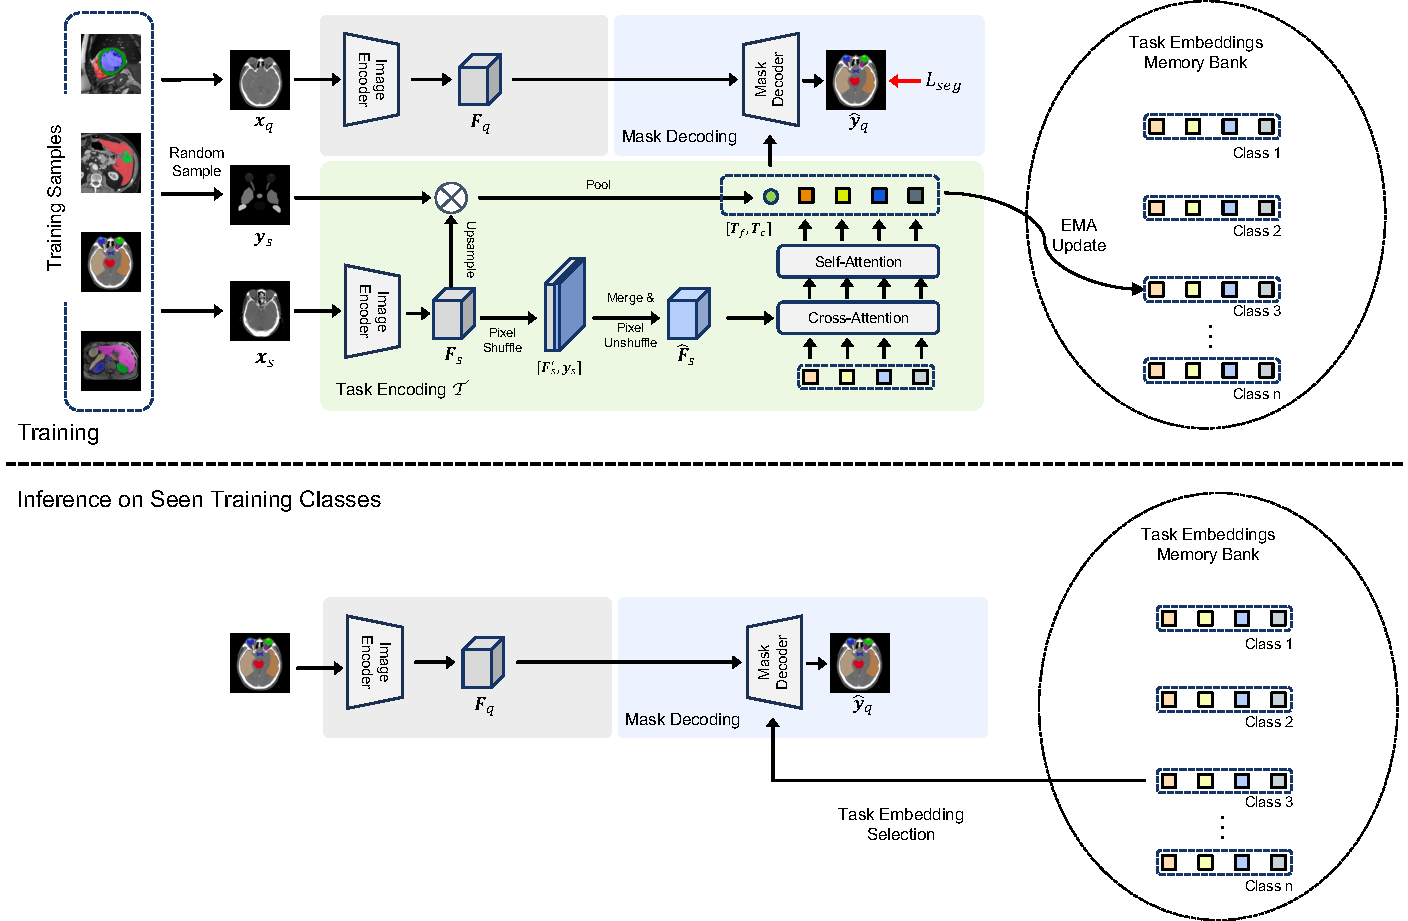
\includegraphics[width=\textwidth]{./fig/supp_context_ensemble.pdf}
\end{center}
\vspace{-1em}
\caption{Context ensemble mechanism for efficient handling of training classes. During training, we maintain a memory bank of class-specific task embeddings, updated via exponential moving average (EMA) whenever a class appears in training iterations. At inference, the model directly selects task embeddings from the memory bank for seen classes, eliminating the need for reference examples while maintaining robust performance through accumulated class knowledge.}
\label{fig:supp_context_ensemble}
\vspace{-1em}
\end{figure*}


\noindent\textbf{Network Architecture.} Our network backbone consists of a 3D UNet with residual connections, comprising four downsampling stages with a base channel dimension of 32. The encoder progressively reduces spatial dimensions while increasing feature channels, and the decoder reconstructs spatial details through skip connections. This architecture effectively captures both local anatomical details and global contextual information in volumetric medical data.

\noindent\textbf{Data Preprocessing.} We implement a standardized preprocessing pipeline to handle the heterogeneous nature of multi-source medical imaging data. First, all volumes are spatially standardized by aligning to a common coordinate system and resampling to an isotropic spacing of $1.5\times 1.5 \times 1.5\ mm$. Intensity normalization is modality-specific: CT images are clipped to the Hounsfield unit range of [-990, 500], while MR and PET images are clipped at their 2nd and 98th percentiles. Finally, z-score normalization is applied to each volume to ensure zero mean and unit standard deviation, facilitating stable network training across different imaging protocols and scanners.

\noindent\textbf{Data Augmentation.} We employ a comprehensive set of augmentation strategies to enhance model robustness. Spatial augmentations include random scaling (0.9 to 1.1), rotation ($\pm$10 degrees), and translation, followed by either random or center cropping to the training size of 128$\times$128$\times$128 voxels. For intensity augmentation, we apply several transformations: multiplicative brightness adjustment (0.9 to 1.1), additive brightness shifts ($\sigma$=0.1), gamma correction (0.8 to 1.2), contrast adjustment (0.8 to 1.2), Gaussian blurring ($\sigma$=0.7 to 1.3), and Gaussian noise ($\sigma\leq$0.02). For reference images, we ensure the preservation of annotated regions after augmentation. These augmentations help simulate various imaging conditions and improve the model's generalization capability across different acquisition protocols and image qualities.

\noindent\textbf{Training and Evaluation Protocol.} During training, Iris processes volumetric data at a window size of $128\times128\times128$ voxels, with random cropping applied as part of our data augmentation strategy to enhance model robustness. For evaluation on large 3D images that exceed the training volume size, we employ a sliding-window inference approach similar to nnUNet~\cite{isensee2021nnu}. This involves moving a $128\times128\times128$ window across the full volume with a 50\% overlap between adjacent windows. Predictions in overlapping regions are averaged to produce smoother segmentation boundaries and reduce edge artifacts. After processing the entire 3D volume, we compute all evaluation metrics (Dice score, etc.) on the complete 3D segmentation result rather than on individual patches, ensuring a comprehensive assessment of the model's performance on anatomical structures of varying sizes and shapes.